\documentclass[preprint,12pt]{elsarticle}

\usepackage{amsmath}
\usepackage{booktabs}
\usepackage{graphicx}
\usepackage{placeins}
\usepackage[T1]{fontenc}
\usepackage[utf8]{inputenc}

\setlength{\emergencystretch}{2em}
\AtBeginEnvironment{thebibliography}{\raggedright\sloppy}

\journal{Internet of Things}

% Generated by scripts/41_build_manuscript_assets.py
\newcommand{\FrozenFprTarget}{1\%}
\newcommand{\NoveltyCoverageFloor}{0.80}
\newcommand{\SourceCompetenceTprFloor}{0.10}
\newcommand{\SourceCompetenceFprCeiling}{0.05}
\newcommand{\DatasetCount}{3}
\newcommand{\DirectionCount}{6}
\newcommand{\ModelCount}{4}
\newcommand{\NaturalSettingCount}{24}
\newcommand{\PrimaryIotSettingCount}{8}
\newcommand{\CompetentSourcePairCount}{9}
\newcommand{\NonCompetentSourcePairCount}{3}
\newcommand{\CompetentSettingCount}{18}
\newcommand{\CompetentRankingFailureCount}{15}
\newcommand{\CompetentCollapseCount}{14}
\newcommand{\CompetentInversionCount}{14}
\newcommand{\CompetentRobustInversionCount}{13}
\newcommand{\CompetentSourcePositiveMedianGapCount}{18}
\newcommand{\CompetentInversionMedianCrossoverCount}{12}
\newcommand{\CompetentIotOnlySettingCount}{6}
\newcommand{\CompetentIotOnlyRankingFailureCount}{3}
\newcommand{\CompetentIotOnlyNonCollapsedCount}{3}
\newcommand{\CompetentUnswStressTestSettingCount}{12}
\newcommand{\CompetentUnswStressTestRankingFailureCount}{12}
\newcommand{\FullRankingFailureCount}{20}
\newcommand{\FullCollapseCount}{19}
\newcommand{\FullInversionCount}{19}
\newcommand{\FullRobustInversionCount}{18}
\newcommand{\FullSourcePositiveMedianGapCount}{24}
\newcommand{\FullInversionMedianCrossoverCount}{17}
\newcommand{\ThresholdDriftCount}{2}
\newcommand{\UnswTargetSettingCount}{8}
\newcommand{\UnswTargetRankingFailureCount}{8}
\newcommand{\TonToIotRankingFailureCount}{3}
\newcommand{\CompetentMinTargetAuroc}{0.249}
\newcommand{\CompetentMaxTargetAuroc}{0.636}
\newcommand{\CompetentTargetPaucMedian}{0.498}
\newcommand{\CompetentTargetPaucMin}{0.497}
\newcommand{\CompetentTargetPaucMax}{0.535}
\newcommand{\CompetentSourcePaucMedian}{0.877}
\newcommand{\CompetentNonCollapsedCount}{3}
\newcommand{\CompetentNonCollapsedTargetPaucMin}{0.500}
\newcommand{\CompetentNonCollapsedTargetPaucMax}{0.507}
\newcommand{\CompetentNonCollapsedSourcePaucMedian}{0.909}
\newcommand{\CompetentMedianTargetTpr}{0.165}
\newcommand{\CompetentMedianRealizedFpr}{0.276}
\newcommand{\CompetentSourceFprMin}{0.004}
\newcommand{\CompetentSourceFprMax}{0.010}
\newcommand{\RecalibrationEvalFprMax}{0.022}
\newcommand{\RecalibrationEvalFprExceedanceCount}{9}
\newcommand{\RecalibrationPartitionScoreKsMedian}{0.013}
\newcommand{\RecalibrationPartitionScoreKsMax}{0.292}
\newcommand{\CatastrophicAllNaturalCount}{17}
\newcommand{\CatastrophicPrimaryIotCount}{6}
\newcommand{\WithinHoldoutMin}{0.000}
\newcommand{\WithinHoldoutMax}{0.996}
\newcommand{\AllNaturalMedianTargetTpr}{0.090}
\newcommand{\AllNaturalMedianRealizedFpr}{0.184}
\newcommand{\AllNaturalMinTargetTpr}{0.000}
\newcommand{\AllNaturalMaxTargetTpr}{0.948}
\newcommand{\AllNaturalMinRealizedFpr}{0.000}
\newcommand{\AllNaturalMaxRealizedFpr}{0.919}
\newcommand{\PrimaryOracleSpearman}{0.436}
\newcommand{\DirectionOracleSpearman}{0.926}
\newcommand{\DirectionBenignKsFprSeveritySpearman}{-0.359}
\newcommand{\IotToTonOracleAlpha}{0.426}
\newcommand{\IotToTonMeanRelativeTprDrop}{0.708}
\newcommand{\IotToTonMeanTargetTpr}{0.166}
\newcommand{\IotToTonMeanRealizedFpr}{0.093}
\newcommand{\TonToIotOracleAlpha}{0.000}
\newcommand{\TonToIotMeanRelativeTprDrop}{0.276}
\newcommand{\TonToIotMeanTargetTpr}{0.693}
\newcommand{\TonToIotMeanRealizedFpr}{0.645}
\newcommand{\IotPairMeanKs}{0.26}
\newcommand{\UnswDirectionMeanKsMin}{0.48}
\newcommand{\UnswDirectionMeanKsMax}{0.54}
\newcommand{\AlphaHatAllNaturalCatastrophicAuroc}{0.403}
\newcommand{\AlphaHatAllNaturalCatastrophicAuprc}{0.696}
\newcommand{\AlphaHatAllNaturalSeveritySpearman}{-0.184}
\newcommand{\ProxyAAllNaturalCatastrophicAuroc}{0.349}
\newcommand{\ProxyAAllNaturalCatastrophicAuprc}{0.665}
\newcommand{\ProxyAAllNaturalSeveritySpearman}{-0.228}
\newcommand{\WassersteinAllNaturalCatastrophicAuroc}{0.382}
\newcommand{\SourceRiskAllNaturalCatastrophicAuroc}{0.492}
\newcommand{\AlphaHatPrimaryCatastrophicAuroc}{0.500}
\newcommand{\AlphaHatPrimarySeveritySpearman}{-0.078}
\newcommand{\SourceRiskPrimaryCatastrophicAuroc}{0.333}
\newcommand{\AllNaturalMedianRetunedTargetTpr}{0.002}
\newcommand{\AllNaturalMedianRetunedTprGain}{-0.078}
\newcommand{\IotToTonMedianRetunedTprGain}{-0.048}
\newcommand{\TonToIotMedianRetunedTprGain}{-0.907}
\newcommand{\BudgetHalfPctMedianTargetTpr}{0.047}
\newcommand{\BudgetOnePctMedianTargetTpr}{0.090}
\newcommand{\BudgetFivePctMedianTargetTpr}{0.292}
\newcommand{\BudgetHalfPctMedianRealizedFpr}{0.148}
\newcommand{\BudgetOnePctMedianRealizedFpr}{0.184}
\newcommand{\BudgetFivePctMedianRealizedFpr}{0.318}
\newcommand{\BudgetHalfPctCompetentMedianSourceTpr}{0.778}
\newcommand{\BudgetHalfPctCompetentMedianTargetTpr}{0.080}
\newcommand{\BudgetHalfPctCompetentMedianTargetRealizedFpr}{0.199}
\newcommand{\BudgetHalfPctCompetentMedianBudgetMultiple}{39.831}
\newcommand{\BudgetHalfPctCompetentCatastrophicCount}{12}
\newcommand{\BudgetOnePctCompetentMedianSourceTpr}{0.806}
\newcommand{\BudgetOnePctCompetentMedianTargetTpr}{0.165}
\newcommand{\BudgetOnePctCompetentMedianTargetRealizedFpr}{0.276}
\newcommand{\BudgetOnePctCompetentMedianBudgetMultiple}{27.585}
\newcommand{\BudgetOnePctCompetentCatastrophicCount}{12}
\newcommand{\BudgetFivePctCompetentMedianSourceTpr}{0.891}
\newcommand{\BudgetFivePctCompetentMedianTargetTpr}{0.346}
\newcommand{\BudgetFivePctCompetentMedianTargetRealizedFpr}{0.318}
\newcommand{\BudgetFivePctCompetentMedianBudgetMultiple}{6.351}
\newcommand{\BudgetFivePctCompetentCatastrophicCount}{8}
\newcommand{\BudgetHalfPctCompetentDominantFprxDirection}{TON$\to$I23}
\newcommand{\BudgetOnePctCompetentDominantFprxDirection}{TON$\to$I23}
\newcommand{\BudgetFivePctCompetentDominantFprxDirections}{TON$\to$UNSW and TON$\to$I23}
\newcommand{\BudgetFivePctCompetentCatastrophicShare}{44\%}
\newcommand{\CoralCompetentMedianTargetAuroc}{0.469}
\newcommand{\CoralCompetentRankingFailureCount}{13}
\newcommand{\CoralCompetentMedianTargetPauc}{0.498}
\newcommand{\CoralCompetentMedianBudgetMultiple}{41.699}
\newcommand{\CoralCompetentCatastrophicCount}{14}
\newcommand{\CoralCompetentCatastrophicShare}{78\%}
\newcommand{\CoverageSweepStableFloorMin}{0.50}
\newcommand{\CoverageSweepStableFloorMax}{0.80}
\newcommand{\CoverageSweepEmptyFloor}{0.90}
\newcommand{\CanonicalRunId}{benchmark\_ac1ed34837025ec1}


\begin{document}

\begin{frontmatter}

\title{Decomposing Fixed-Threshold Transfer in Tabular Flow-Level NIDS}

\author{Mustafa Ipekbayrak}
\author{G{\"u}ls{\"u}m Zeynep G{\"u}rka\c{s}-Ayd{\i}n}

\begin{abstract}
Cross-dataset evaluations of network intrusion detection systems (NIDS) routinely show degradation under domain shift, but they seldom distinguish threshold miscalibration from loss of ranking quality. We study this distinction in a three-corpus benchmark of fixed-threshold transfer for tabular flow-level NIDS using IoT-23, ToN-IoT, and UNSW-NB15. All corpora are mapped to a shared 16-feature flow schema, \ModelCount{} tabular classifiers are trained, and thresholds selected on source validation at \FrozenFprTarget{} false positive rate are transferred unchanged. Of \NaturalSettingCount{} transfer settings, \CompetentSettingCount{} pass a predeclared source-competence filter. Among these \CompetentSettingCount{} competent settings, \CompetentRankingFailureCount{} fall below target AUROC 0.60, and \CompetentInversionCount{} of those failures are below chance on point estimates under the transferred score orientation. The benchmark-wide count is driven by the \CompetentUnswStressTestSettingCount{} UNSW-related stress-test directions; the \CompetentIotOnlySettingCount{} IoT-only competent transfers split \CompetentIotOnlyRankingFailureCount{} failures and \CompetentIotOnlyNonCollapsedCount{} rows above the 0.60 failure floor. Low-FPR ranking is near chance benchmark-wide: target standardized pAUC@1\% ranges from \CompetentTargetPaucMin{} to \CompetentTargetPaucMax{} (median \CompetentTargetPaucMedian{}), compared with a source-holdout median of \CompetentSourcePaucMedian{}. Benign-only threshold reselection does not rescue detection (mean recalibrated TPR 0.013 across all \NaturalSettingCount{} settings), and neither a 0.5\%/1\%/5\% source-side budget sweep nor an auxiliary CORAL comparison changes the deployment conclusion at the chosen budget. In this three-corpus benchmark, cross-dataset degradation is therefore dominated by ranking failure rather than threshold drift. Secondary analyses of attack novelty, benign covariate shift, and target-free monitors remain limited, and none of the audited monitors is reliable enough for deployment.
\end{abstract}

\begin{keyword}
IoT intrusion detection \sep domain shift \sep cross-dataset evaluation \sep false positive control \sep ranking failure \sep target-free monitoring
\end{keyword}

\end{frontmatter}

\section{Introduction}

The instability of operating points across network domains has been a foundational concern in security machine learning since Axelsson~\cite{axelsson2000baserate} quantified the base-rate fallacy and Sommer and Paxson~\cite{sommer2010outside} argued that closed-world evaluations systematically overstate classifier utility. What remains missing is a direct operational decomposition: when a threshold trained in one network is deployed unchanged in another, what fails, and which component of the shift drives it?

Prior cross-dataset evaluations have shown that IDS models lose generalization strength under domain change~\cite{dhooge2020inter,layeghy2024benchmarking,iwanowski2025choice}. These studies document the existence of degradation without decomposing it. In particular, they do not distinguish between two operationally different failure modes: \emph{ranking failure}, in which the transferred score direction no longer yields enough target discrimination for operational repair, and \emph{threshold drift}, in which the model's ranking is preserved but the source-calibrated operating point falls in the wrong region of the target's score distribution. In the taxonomy used here, ranking failure is later split into ranking collapse (AUROC~$\leq$~0.50) and ranking degradation (0.50~$<$~AUROC~$<$~0.60); below-chance rows are the inverted-orientation subset of collapse. The distinction matters because ranking failure is not fixed by simple threshold movement, while threshold drift can in principle be repaired by recalibration on unlabeled target data.

This paper addresses the decomposition gap in a three-corpus benchmark. It builds a fixed-threshold cross-dataset benchmark across IoT-23, ToN-IoT, and UNSW-NB15 using one shared tabular feature schema and \ModelCount{} practical classifiers. Each threshold is frozen on source validation at \FrozenFprTarget{} false positive rate and transferred unchanged to every target domain, producing \NaturalSettingCount{} natural-transfer settings. It then decomposes each setting's failure into three components:

\begin{enumerate}
    \item \textbf{Ranking failure:} Whether the target AUROC falls below a floor that makes threshold repair operationally insufficient, with collapse and degradation subtypes (Section~\ref{sec:ranking-diagnosis}).
    \item \textbf{Attack-label novelty:} Whether novel attack types unseen in the source training set explain target sensitivity loss, measured via oracle novelty $\alpha$ on the claim-bearing IoT subset (Section~\ref{sec:oracle-novelty}).
    \item \textbf{Benign covariate shift:} Whether distributional drift in the benign feature space drives false-positive inflation independently of attack novelty (Section~\ref{sec:covariate-shift}).
\end{enumerate}

The paper contributes three empirical findings. First, the dominant failure mode in this three-corpus benchmark is ranking failure: \FullRankingFailureCount{} of \NaturalSettingCount{} settings have target AUROC below 0.60. On point estimates, \FullInversionCount{} of those failing settings fall strictly below chance, indicating inverted target score orientation under the transferred rule. This benchmark-wide result includes the Tier~1 stress-test directions involving UNSW-NB15, while the claim-bearing novelty analysis remains restricted to the \PrimaryIotSettingCount{} IoT-only settings. Second, on that claim-bearing IoT subset, oracle novelty provides only a bounded directional explanation of sensitivity loss (subset Spearman \PrimaryOracleSpearman{}), while the global benign-shift association with false-positive severity remains weak and non-monotone (Spearman $\DirectionBenignKsFprSeveritySpearman{}$ over \DirectionCount{} directions). Third, the pre-registered target-free novelty proxy $\hat{\alpha}$ remains too weak for operational deployment on the full benchmark (catastrophic-failure AUROC \AlphaHatAllNaturalCatastrophicAuroc{}).

\section{Related Work}

Operational evaluation in intrusion detection has long required more than global ranking summaries. ROC and precision-recall curves remain useful, but they do not replace reporting at the false positive budget that governs deployment~\cite{axelsson2000baserate,fawcett2006roc,davis2006pr}. That matters even more in network security, where dataset construction, capture conditions, label quality, and traffic mix vary sharply across corpora~\cite{ring2019survey}.

The move from within-dataset modeling to cross-dataset evaluation is therefore central to realistic IDS assessment. Prior work has shown that intrusion-detection models often lose substantial generalization strength once the training and evaluation datasets differ in their traffic and attack composition~\cite{sommer2010outside,dhooge2020inter,layeghy2024benchmarking,iwanowski2025choice}. Recent cross-domain evaluations make the same point from a model-centric angle: transfer behavior can change sharply across datasets even when within-domain performance is strong~\cite{ring2019survey}.

The monitoring question is adjacent but distinct. Under domain shift, unlabeled diagnostics such as domain-classifier distances or feature-distribution distances are often used as rough warnings, while predictive confidence and uncertainty are known to degrade under shift in ways that are hard to trust without direct validation~\cite{ben2010domain,ovadia2019uncertainty,rabanser2019failing,hendrycks2017baseline}. This paper treats monitoring as a secondary audit of the same fixed-threshold transfer protocol rather than as a new monitoring method. It compares one pre-registered novelty proxy against simple unlabeled baselines and reports the negative result when the proxy does not justify a stronger operational claim.

\section{Study Design}

\subsection{Datasets and Tiered Analysis}

The benchmark uses three public datasets arranged in two tiers. \emph{Tier~1} (full benchmark) includes all three datasets---IoT-23, ToN-IoT, and UNSW-NB15~\cite{garcia2020iot23,booij2022ton,moustafa2015unsw}---across all \DirectionCount{} ordered source-target directions, yielding \NaturalSettingCount{} transfer settings. All benchmark metrics (TPR, FPR, AUROC, AUPRC, ranking diagnosis) are reported on Tier~1. \emph{Tier~2} (claim-bearing novelty subset) restricts to the \PrimaryIotSettingCount{} IoT-only settings (IoT-23~$\leftrightarrow$~ToN-IoT) where the coarse attack ontology achieves mapped attack coverage above \NoveltyCoverageFloor{} on both domains. Oracle novelty claims are made only on Tier~2. UNSW-NB15 is retained in Tier~1 as a stress-test domain that reveals how severe ranking failure becomes under large covariate and label-space gaps, but it is not treated as a semantic peer in the novelty analysis because the current coarse ontology does not cover its attack taxonomy well enough.

\subsection{Feature Schema and Preprocessing}

All three datasets are mapped into one shared primitive schema consisting of record\_id, group\_id, label, family\_raw, proto, duration\_s, src\_bytes, dst\_bytes, src\_pkts, and dst\_pkts. The canonical feature representation is the generated shared schema feature\_schema\_v1.

% Generated by src/iot_ids/schema_appendix.py
\begin{table}[!tbp]
\centering
\footnotesize
\renewcommand{\arraystretch}{1.08}
\setlength{\tabcolsep}{4pt}
\caption{Shared-schema quantitative features used in the canonical benchmark (feature schema v1).}
\label{tab:shared-feature-schema-quantitative}
\begin{tabular}{p{0.22\columnwidth}p{0.42\columnwidth}p{0.18\columnwidth}}
\toprule
Feature & Formula & Derived From \\
\midrule
\begin{tabular}[t]{@{}l@{}}log\_duration\_ \\ s\end{tabular} & log1p(max(duration\_s, 0)) & duration\_s \\
\begin{tabular}[t]{@{}l@{}}log\_src\_ \\ bytes\end{tabular} & log1p(max(src\_bytes, 0)) & src\_bytes \\
\begin{tabular}[t]{@{}l@{}}log\_dst\_ \\ bytes\end{tabular} & log1p(max(dst\_bytes, 0)) & dst\_bytes \\
\begin{tabular}[t]{@{}l@{}}log\_src\_ \\ pkts\end{tabular} & log1p(max(src\_pkts, 0)) & src\_pkts \\
\begin{tabular}[t]{@{}l@{}}log\_dst\_ \\ pkts\end{tabular} & log1p(max(dst\_pkts, 0)) & dst\_pkts \\
\begin{tabular}[t]{@{}l@{}}log\_total\_ \\ bytes\end{tabular} & \begin{tabular}[t]{@{}l@{}}log1p(src\_bytes + \\ dst\_bytes)\end{tabular} & \begin{tabular}[t]{@{}l@{}}src\_bytes, \\ dst\_bytes\end{tabular} \\
\begin{tabular}[t]{@{}l@{}}log\_total\_ \\ pkts\end{tabular} & \begin{tabular}[t]{@{}l@{}}log1p(src\_pkts + \\ dst\_pkts)\end{tabular} & \begin{tabular}[t]{@{}l@{}}src\_pkts, \\ dst\_pkts\end{tabular} \\
\begin{tabular}[t]{@{}l@{}}log\_bytes\_ \\ per\_s\end{tabular} & \begin{tabular}[t]{@{}l@{}}log1p((src\_bytes + \\ dst\_bytes) \\ / duration\_s); \\ 0 when duration\_s = 0\end{tabular} & \begin{tabular}[t]{@{}l@{}}duration\_s, \\ src\_bytes, \\ dst\_bytes\end{tabular} \\
\begin{tabular}[t]{@{}l@{}}log\_pkts\_ \\ per\_s\end{tabular} & \begin{tabular}[t]{@{}l@{}}log1p((src\_pkts + \\ dst\_pkts) \\ / duration\_s); \\ 0 when duration\_s = 0\end{tabular} & \begin{tabular}[t]{@{}l@{}}duration\_s, \\ src\_pkts, \\ dst\_pkts\end{tabular} \\
\begin{tabular}[t]{@{}l@{}}src\_byte\_ \\ frac\end{tabular} & \begin{tabular}[t]{@{}l@{}}src\_bytes \\ / (src\_bytes + \\ dst\_bytes); \\ 0.5 when total\_bytes = 0\end{tabular} & \begin{tabular}[t]{@{}l@{}}src\_bytes, \\ dst\_bytes\end{tabular} \\
\begin{tabular}[t]{@{}l@{}}src\_pkt\_ \\ frac\end{tabular} & \begin{tabular}[t]{@{}l@{}}src\_pkts \\ / (src\_pkts + \\ dst\_pkts); \\ 0.5 when total\_pkts = 0\end{tabular} & \begin{tabular}[t]{@{}l@{}}src\_pkts, \\ dst\_pkts\end{tabular} \\
\begin{tabular}[t]{@{}l@{}}bytes\_per\_ \\ pkt\end{tabular} & \begin{tabular}[t]{@{}l@{}}(src\_bytes + \\ dst\_bytes) \\ / (src\_pkts + \\ dst\_pkts); \\ 0 when total\_pkts = 0\end{tabular} & \begin{tabular}[t]{@{}l@{}}src\_bytes, \\ dst\_bytes, \\ src\_pkts, \\ dst\_pkts\end{tabular} \\
\bottomrule
\end{tabular}
\end{table}

\FloatBarrier

Table~\ref{tab:shared-feature-schema-quantitative} lists the 12 quantitative derived features. The protocol field is one-hot encoded into four canonical indicators: proto\_tcp, proto\_udp, proto\_icmp, and proto\_other. The per-dataset raw-to-primitive mapping rules and discarded staged columns remain in the generated artifact package for reproducibility. No dataset-specific feature branch is allowed in the canonical run. That choice constrains model capacity, but it preserves comparability across all source-target directions.

\subsection{Source-Only Protocol and Threshold Freezing}

Each source dataset is split deterministically into train, validation, and source-holdout partitions. Source-fitted preprocessing is then applied unchanged to the source holdout and to every transferred target dataset. The benchmark trains \ModelCount{} practical tabular classifiers spanning linear, ensemble, and neural settings, without introducing model shopping or hyperparameter sweeps. For each source-model pair, the threshold is fixed once on source validation negatives at \FrozenFprTarget{} false positive rate and is transferred unchanged to every target evaluation. Predictions are defined by the tie-safe rule score $\geq$ threshold. The selected threshold is the smallest cutoff whose realized FPR under that rule does not exceed the budget; if a tied block of negative scores straddles the budget, the cutoff is moved strictly above the tied score so those tied negatives remain negative. To test whether the deployment conclusion is tied to the nominal operating point, the same frozen source-threshold transfer protocol is additionally audited at 0.5\%, 1\%, and 5\% source-validation FPR budgets, transferring each source-selected threshold unchanged to source holdout and target. As one auxiliary unlabeled adaptation check, CORAL is fit using source-train features and a deterministic 50/50 target-test adaptation half split by group, then evaluated on the disjoint target-evaluation half under the same frozen \FrozenFprTarget{} source-validation threshold rule.

\subsection{Transfer Metrics}

The main within-domain quantity is source-holdout TPR at the frozen operating point. The main transfer quantities are target TPR at that same operating point, realized target false positive rate, AUROC, AUPRC, and signed relative TPR change,
\[
\Delta_{\mathrm{TPR,rel}} = \frac{\mathrm{TPR}_{\mathrm{target}}}{\max(\mathrm{TPR}_{\mathrm{source\ holdout}}, \varepsilon)} - 1.
\]
Negative values indicate transferred sensitivity loss, while positive values indicate target sensitivity above the source holdout. When the paper needs a nonnegative degradation summary, it reports relative TPR drop, defined as $\max(-\Delta_{\mathrm{TPR,rel}}, 0)$. Because the source and target domains are unmatched, the benchmark is descriptive and does not use cross-domain paired significance testing.

\subsection{Oracle Novelty}

Oracle novelty, denoted $\alpha$, is defined with target labels and a coarse attack ontology. For a given source-target setting,
\[
\alpha = \frac{\sum_{i=1}^{n_t}\mathbf{1}[g_i \notin G_s]}{n_t},
\]
where $G_s$ is the set of source attack ontology groups, $g_i$ are the target attack ontology groups, and both source and target exclude the group other. The novelty analysis is treated as claim-bearing only when both source and target mapped attack coverage reach at least \NoveltyCoverageFloor{}. Under the current ontology this leaves \PrimaryIotSettingCount{} IoT-only settings as the primary novelty subset and excludes the UNSW-NB15 directions from novelty claims.

It is important to note that $\alpha$ measures label-space overlap, not feature-space proximity. Performance drop can occur without label novelty (via covariate shift in benign traffic) and need not occur despite high novelty (if novel attack types behave similarly to seen types in feature space). The correlation between $\alpha$ and transfer degradation is therefore an empirical finding, not a definitional tautology.

\subsection{Target-Free Monitors}
\label{sec:monitors}

The benchmark compares four unlabeled transfer monitors, each computable without target labels:

\paragraph{Target-free novelty proxy ($\hat{\alpha}$).} The proxy is frozen before the full benchmark is read. It uses source-train attack instances after the source-fitted standardized preprocessing path, fits a $k$-nearest-neighbor model with $k=10$, and sets the cutoff distance at the $0.95$ quantile of the leave-one-out source-attack distances. At transfer time, it selects target instances predicted positive by the frozen detector threshold. If no target instance is predicted positive, it uses the top-$K$ target instances by detector score, where $K=\lceil q_{\text{src-val-pos}} n_{\text{target}}\rceil$ and $q_{\text{src-val-pos}}$ is the positive prediction rate on source validation under the frozen threshold. The proxy is then the fraction of selected target instances whose $k$-nearest-neighbor distance to the source attack bank exceeds the source cutoff.

\paragraph{Proxy-A distance ($d_A$).} A source-versus-target logistic domain classifier is trained on a held-out split using logistic regression with the liblinear solver. The held-out classification error $\mathrm{err}$ measures how separable the two domains are in feature space. The distance is $d_A = \max(0, 2(1 - 2\,\mathrm{err}))$. Higher values indicate greater distributional distance between source and target features, suggesting that the model's learned decision boundary may not transfer.

\paragraph{Wasserstein distance.} For each feature, the one-dimensional Wasserstein distance is the mean absolute difference between matched empirical quantiles of the source-train and target distributions. The monitor then averages these distances across features. This captures marginal distributional shift without learning a domain classifier.

\paragraph{Source-validation risk.} The negated source-validation TPR at the frozen operating point, $-\mathrm{TPR}_{\mathrm{src\text{-}val}}$. This trivial baseline encodes the prior that weaker source-side detection quality correlates with worse transfer. It requires no target data beyond the threshold itself and serves as a floor comparator.

For monitor evaluation, the paper uses an operational severity score that combines sensitivity loss and false-positive drift: $\mathrm{fpr\_budget\_multiple} = \mathrm{FPR}_{\mathrm{target}} / 0.01$, $\mathrm{fpr\_severity} = \min\!\left(1, \max(0, \mathrm{fpr\_budget\_multiple} - 1) / 9\right)$, and $\mathrm{operational\_severity} = \max(\mathrm{relative\_TPR\_drop}, \mathrm{fpr\_severity})$. The secondary binary monitor target is catastrophic operational failure, defined as $\mathrm{catastrophic} = 1(\mathrm{operational\_severity} \geq 1)$.

\section{Results}

\subsection{Within-Domain Sanity}

This subsection establishes that the source models are meaningful before transfer, while also showing that source-side strength varies sharply across datasets and model classes. Source-holdout TPR at the frozen operating point ranges from \WithinHoldoutMin{} to \WithinHoldoutMax{}.

The spread already warns against reading source performance as a deployment surrogate. HistGradientBoosting is strong on IoT-23 and ToN-IoT, logistic regression is weak on ToN-IoT, and Extra-Trees is frozen-threshold blind on IoT-23 and UNSW-NB15. The within-domain table marks these weak source rows explicitly so they are not mistaken for competent transfer candidates.

% Generated by scripts/41_build_manuscript_assets.py
\begin{table}[htbp]
\centering
\small
\setlength{\tabcolsep}{4pt}
\caption{Within-domain source-side performance under the frozen \FrozenFprTarget{} source-validation operating point. Confidence intervals are grouped-bootstrap percentile intervals over group identifiers. Rows marked with $\dagger$ fail the source-side competence rule used for the competent-setting subset.}
\label{tab:within-domain}
\resizebox{\textwidth}{!}{%
\begin{tabular}{llrlrl}
\toprule
Dataset & Model & Source holdout TPR@\FrozenFprTarget{} & 95\% CI & Source validation TPR@\FrozenFprTarget{} & 95\% CI  \\
\midrule
IoT-23 & LR & 0.521 & [0.519, 0.522] & 0.523 & [0.521, 0.524] \\
 & ET$\dagger$ & 0.000 & [0.000, 0.000] & 0.000 & [0.000, 0.000] \\
 & HGB & 0.953 & [0.953, 0.954] & 0.954 & [0.954, 0.955] \\
 & MLP & 0.773 & [0.772, 0.774] & 0.776 & [0.774, 0.777] \\
ToN-IoT & LR$\dagger$ & 0.080 & [0.076, 0.085] & 0.081 & [0.076, 0.086] \\
 & ET & 0.996 & [0.993, 0.998] & 0.997 & [0.996, 0.998] \\
 & HGB & 0.993 & [0.989, 0.995] & 0.994 & [0.993, 0.995] \\
 & MLP & 0.968 & [0.964, 0.971] & 0.970 & [0.968, 0.973] \\
UNSW-NB15 & LR & 0.245 & [0.241, 0.250] & 0.245 & [0.240, 0.250] \\
 & ET$\dagger$ & 0.000 & [0.000, 0.000] & 0.000 & [0.000, 0.000] \\
 & HGB & 0.806 & [0.802, 0.811] & 0.808 & [0.804, 0.812] \\
 & MLP & 0.624 & [0.619, 0.629] & 0.621 & [0.616, 0.626] \\
\bottomrule
\end{tabular}
}
\end{table}


That variation matters because it does not map cleanly onto transferred behavior. The source-side table is therefore a sanity check rather than a claim about deployment quality. The next subsection turns to the benchmark that answers that deployment question directly.

\FloatBarrier

\subsection{Full Cross-Domain Transfer Benchmark}

This subsection reports the full Tier~1 benchmark: \NaturalSettingCount{} settings formed by \DirectionCount{} ordered source-target directions and \ModelCount{} models. Across those settings, median target TPR at the frozen operating point is \AllNaturalMedianTargetTpr{}, while median realized false positive rate is \AllNaturalMedianRealizedFpr{}. The full range is wider still, with target TPR spanning \AllNaturalMinTargetTpr{} to \AllNaturalMaxTargetTpr{} and realized false positive rate spanning \AllNaturalMinRealizedFpr{} to \AllNaturalMaxRealizedFpr{}.

Figures~\ref{fig:transfer-tpr} and~\ref{fig:transfer-fpr} together with Table~\ref{tab:cross-domain} show the same operational point from complementary views. The transferred operating point is not stable. In the IoT-23 to ToN-IoT direction, logistic regression preserves moderate target sensitivity only by drifting to a much higher benign alert rate, whereas the tree models stay near the nominal false positive budget and almost stop detecting attacks. In the reverse ToN-IoT to IoT-23 direction, the stronger transferred models retain high target sensitivity but do so with realized false positive rates far above the intended operating point. The stress-test directions involving UNSW-NB15 remain in Tier~1 because they show how severe this instability can become even when novelty claims are out of scope.

\begin{figure}[t]
\centering
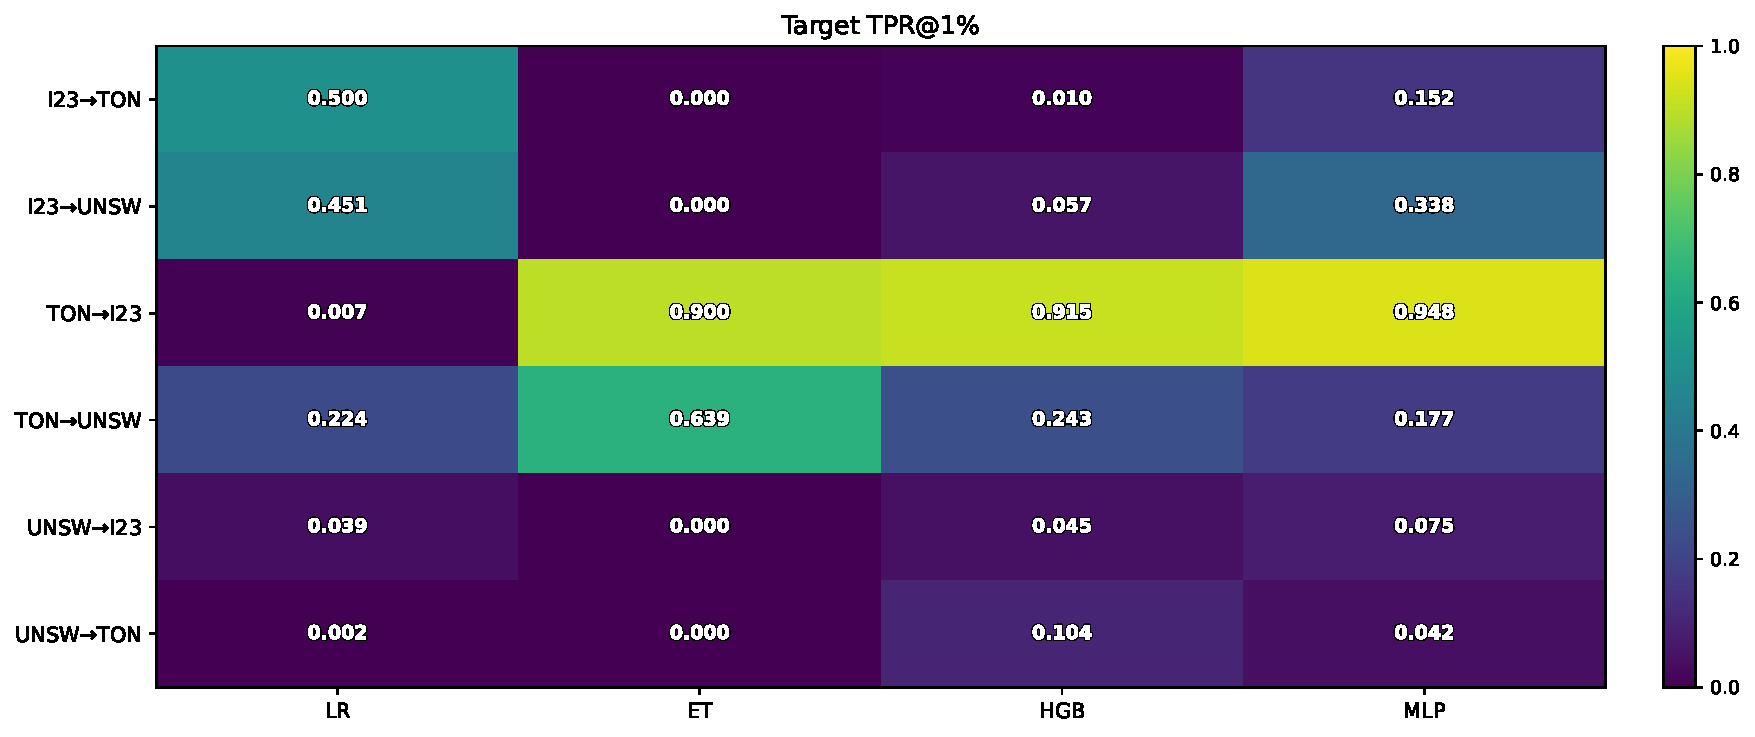
\includegraphics[width=\textwidth]{figures/transfer_tpr.pdf}
\caption{Tier~1 benchmark: target TPR at the frozen \FrozenFprTarget{} operating point.}
\label{fig:transfer-tpr}
\end{figure}

\begin{figure}[t]
\centering
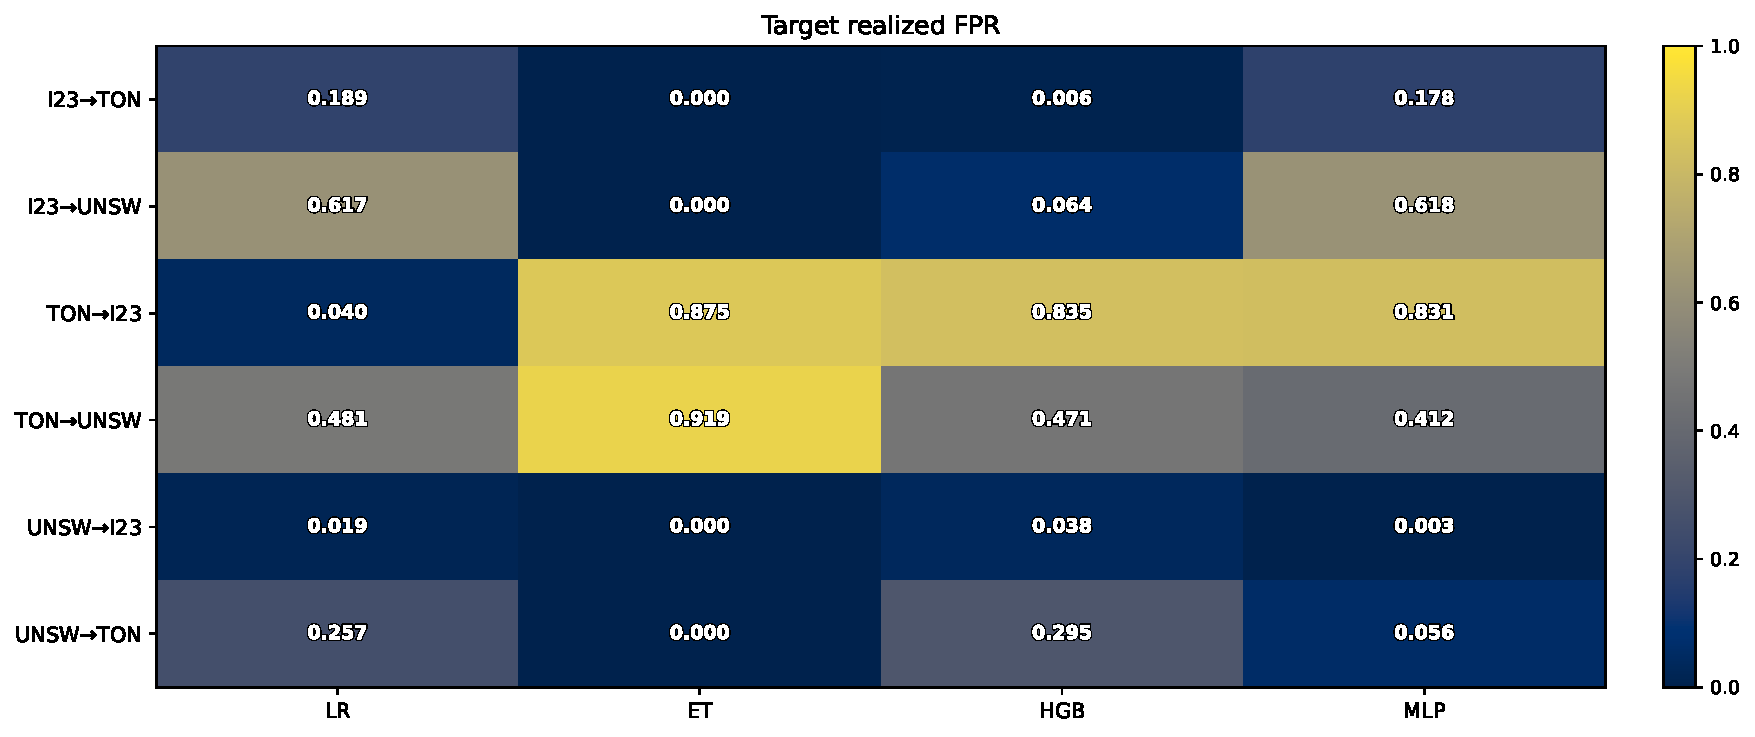
\includegraphics[width=\textwidth]{figures/transfer_fpr.pdf}
\caption{Tier~1 benchmark: realized target false positive rate under the transferred threshold.}
\label{fig:transfer-fpr}
\end{figure}

% Generated by scripts/41_build_manuscript_assets.py
\begin{table}[htbp]
\centering
\footnotesize
\setlength{\tabcolsep}{4pt}
\caption{Cross-domain fixed-threshold benchmark across all \NaturalSettingCount{} transfer settings. Confidence intervals are grouped-bootstrap percentile intervals over group identifiers. Rows marked as stress-test remain in the operational benchmark but are excluded from claim-bearing oracle novelty interpretation.}
\label{tab:cross-domain}
\resizebox{\textwidth}{!}{%
\begin{tabular}{lllrlrrrrll}
\toprule
Source & Target & Model & TPR@\FrozenFprTarget{} & 95\% CI & Realized FPR & 95\% CI  & AUROC & AUPRC & Relative TPR drop & Scope \\
\midrule
IoT-23 & ToN-IoT & LR & 0.500 & [0.480, 0.520] & 0.189 & [0.117, 0.294] & 0.636 & 0.765 & 0.040 & primary \\
 &  & ET & 0.000 & [0.000, 0.000] & 0.000 & [0.000, 0.000] & 0.633 & 0.800 & 1.000 & primary \\
 &  & HGB & 0.010 & [0.009, 0.011] & 0.006 & [0.004, 0.011] & 0.617 & 0.801 & 0.990 & primary \\
 &  & MLP & 0.152 & [0.143, 0.162] & 0.178 & [0.110, 0.274] & 0.559 & 0.723 & 0.803 & primary \\
 & UNSW-NB15 & LR & 0.451 & [0.446, 0.457] & 0.617 & [0.610, 0.624] & 0.360 & 0.539 & 0.133 & stress-test \\
 &  & ET & 0.000 & [0.000, 0.000] & 0.000 & [0.000, 0.000] & 0.347 & 0.592 & 1.000 & stress-test \\
 &  & HGB & 0.057 & [0.054, 0.059] & 0.064 & [0.061, 0.067] & 0.407 & 0.633 & 0.941 & stress-test \\
 &  & MLP & 0.338 & [0.333, 0.343] & 0.618 & [0.610, 0.625] & 0.329 & 0.542 & 0.562 & stress-test \\
\midrule
ToN-IoT & IoT-23 & LR & 0.007 & [0.007, 0.008] & 0.040 & [0.038, 0.043] & 0.392 & 0.901 & 0.908 & primary \\
 &  & ET & 0.900 & [0.899, 0.901] & 0.875 & [0.870, 0.879] & 0.453 & 0.928 & 0.096 & primary \\
 &  & HGB & 0.915 & [0.914, 0.916] & 0.835 & [0.831, 0.840] & 0.427 & 0.926 & 0.078 & primary \\
 &  & MLP & 0.948 & [0.947, 0.949] & 0.831 & [0.826, 0.835] & 0.624 & 0.950 & 0.020 & primary \\
 & UNSW-NB15 & LR & 0.224 & [0.219, 0.228] & 0.481 & [0.474, 0.488] & 0.274 & 0.505 & 0.000 & stress-test \\
 &  & ET & 0.639 & [0.634, 0.644] & 0.919 & [0.915, 0.923] & 0.249 & 0.497 & 0.358 & stress-test \\
 &  & HGB & 0.243 & [0.238, 0.247] & 0.471 & [0.464, 0.478] & 0.360 & 0.560 & 0.756 & stress-test \\
 &  & MLP & 0.177 & [0.173, 0.181] & 0.412 & [0.405, 0.419] & 0.258 & 0.500 & 0.817 & stress-test \\
\midrule
UNSW-NB15 & IoT-23 & LR & 0.039 & [0.038, 0.039] & 0.019 & [0.017, 0.021] & 0.418 & 0.919 & 0.843 & stress-test \\
 &  & ET & 0.000 & [0.000, 0.000] & 0.000 & [0.000, 0.000] & 0.444 & 0.905 & 1.000 & stress-test \\
 &  & HGB & 0.045 & [0.045, 0.046] & 0.038 & [0.036, 0.041] & 0.375 & 0.927 & 0.944 & stress-test \\
 &  & MLP & 0.075 & [0.074, 0.076] & 0.003 & [0.002, 0.004] & 0.425 & 0.922 & 0.879 & stress-test \\
 & ToN-IoT & LR & 0.002 & [0.001, 0.002] & 0.257 & [0.150, 0.377] & 0.386 & 0.646 & 0.993 & stress-test \\
 &  & ET & 0.000 & [0.000, 0.000] & 0.000 & [0.000, 0.000] & 0.192 & 0.570 & 1.000 & stress-test \\
 &  & HGB & 0.104 & [0.098, 0.109] & 0.295 & [0.185, 0.450] & 0.285 & 0.627 & 0.871 & stress-test \\
 &  & MLP & 0.042 & [0.040, 0.045] & 0.056 & [0.034, 0.084] & 0.414 & 0.672 & 0.932 & stress-test \\
\bottomrule
\end{tabular}
}
\end{table}


The main result of the paper sits here. High source-side performance does not guarantee transferred operating-point stability, and the failure mode is not one-dimensional. That observation motivates the failure mode decomposition in the next subsection.

\FloatBarrier

\subsection{Failure Mode Decomposition: Ranking Failure versus Threshold Drift}
\label{sec:ranking-diagnosis}

This subsection addresses a question the cross-domain benchmark alone leaves open: \emph{why} does transfer fail? Two operationally different mechanisms can produce a low target TPR at a frozen threshold. First, the model may lose enough target discrimination that the transferred score ordering is no longer operationally usable---\emph{ranking failure}---in which case simple threshold movement cannot recover acceptable detection. Second, the model's ranking may survive the shift but the frozen threshold may land in the wrong region of the target score distribution---\emph{threshold drift}---in which case recalibration on unlabeled target statistics could in principle repair the operating point.

We classify each of the \NaturalSettingCount{} settings by its target AUROC. A setting with target AUROC at or below~0.50 is classified as \emph{ranking collapse}; exact-chance rows are collapse without usable directional signal. A setting with 0.50~$<$~AUROC~$<$~0.60 is classified as \emph{ranking degraded}. Rows with target AUROC below~0.50 indicate the \emph{inverted target score orientation} subset of collapse under the fixed score~$\geq$~threshold rule. No setting in this benchmark lies exactly at the AUROC~=~0.50 boundary. A setting with AUROC at or above~0.60 but large relative TPR drop under the frozen threshold is classified as threshold drift.

% Generated by scripts/41_build_manuscript_assets.py
\begin{table}[htbp]
\centering
\footnotesize
\setlength{\tabcolsep}{4pt}
\caption{Failure-mode decomposition for all \NaturalSettingCount{} natural-transfer settings. The final row is descriptive rather than a success label: it marks rows with target AUROC~$\geq$~0.60 and relative TPR drop~$\leq$~0.50, not operationally acceptable deployment. Collapse rows include both at-chance and inverted-orientation failures under the transferred score direction.}
\label{tab:ranking-diagnosis}
\resizebox{\textwidth}{!}{%
\begin{tabular}{llrrrr}
\toprule
Diagnosis & Criterion & Count & Median target AUROC & Median realized FPR & Median relative TPR drop \\
\midrule
Ranking collapse & AUROC $\leq$ 0.50 & 19 & 0.375 & 0.257 & 0.871 \\
Ranking degraded & 0.50 $<$ AUROC $<$ 0.60 & 1 & 0.559 & 0.178 & 0.803 \\
Threshold drift & AUROC $\geq$ 0.60; drop $>$ 0.50 & 2 & 0.625 & 0.003 & 0.995 \\
Non-collapsed, low TPR loss & AUROC $\geq$ 0.60; drop $\leq$ 0.50 & 2 & 0.630 & 0.510 & 0.030 \\
\bottomrule
\end{tabular}
}
\end{table}


The dominant failure is ranking failure. Across all \NaturalSettingCount{} settings, \FullRankingFailureCount{} fall below target AUROC~0.60. On point estimates, \FullCollapseCount{} of those settings are collapse rows; because no setting lies exactly at the AUROC~=~0.50 boundary, all \FullCollapseCount{} are below-chance inversions under the transferred score orientation. Only \ThresholdDriftCount{} settings exhibit threshold drift with preserved ranking quality. The UNSW-NB15 target directions are uniformly in ranking failure (\UnswTargetRankingFailureCount{} of \UnswTargetSettingCount{} settings). Even within the IoT-only directions, the ToN-IoT~$\to$~IoT-23 direction has \TonToIotRankingFailureCount{} of \ModelCount{} settings in ranking failure.

A score-space view is consistent with that interpretation: all \FullSourcePositiveMedianGapCount{} source-holdout rows keep attack median scores above benign medians, while \FullInversionMedianCrossoverCount{} of the \FullInversionCount{} point-estimate inversion rows show target benign medians meeting or exceeding target attack medians.

This finding has two implications. First, threshold repair strategies---such as recalibrating the operating point on unlabeled target benign statistics---cannot address the dominant failure mode in this benchmark. The failure is in the learned representation, not in the threshold placement. Second, the diagnostic oracle-retuning summary in Appendix~\ref{app:oracle-retuning} points the same way: retuning the threshold on target labels yields median paired TPR change \AllNaturalMedianRetunedTprGain{}, so even with target-label access for threshold selection, the ranking is usually too degraded to recover sensitivity at the frozen budget.

\subsection{Operating-Budget Robustness}
\label{sec:budget-robustness}

% Generated by scripts/41_build_manuscript_assets.py
\begin{table}[htbp]
\centering
\footnotesize
\setlength{\tabcolsep}{3pt}
\caption{Source-selected operating-budget robustness on the 18 competent settings. Each row freezes the threshold at the listed source-validation FPR budget and transfers it unchanged to source holdout and target. Med. realized FPR is the median target false-positive rate under that transferred threshold. FPR$\times$ denotes the median realized target FPR divided by the selected source-side budget. Cat./18 counts catastrophic settings under the existing operational-severity rule.}
\label{tab:budget-robustness}
\resizebox{\textwidth}{!}{%
\begin{tabular}{lrrrrr}
\toprule
Budget & Src holdout med. TPR & Tgt med. TPR & Med. realized FPR & Med. FPR$\times$ & Cat./18 \\
\midrule
0.5\% & 0.778 & 0.080 & 0.199 & 39.831 & 12 \\
1\% & 0.806 & 0.165 & 0.276 & 27.585 & 12 \\
5\% & 0.891 & 0.346 & 0.318 & 6.351 & 8 \\
\bottomrule
\end{tabular}
}
\end{table}


Table~\ref{tab:budget-robustness} shows that loosening the source-selected budget makes the transferred threshold more aggressive: competent-set median source-holdout TPR rises from \BudgetHalfPctCompetentMedianSourceTpr{} to \BudgetFivePctCompetentMedianSourceTpr{}, and median target TPR rises from \BudgetHalfPctCompetentMedianTargetTpr{} to \BudgetFivePctCompetentMedianTargetTpr{}. But median realized target FPR also rises from \BudgetHalfPctCompetentMedianTargetRealizedFpr{} to \BudgetFivePctCompetentMedianTargetRealizedFpr{}, which still corresponds to \BudgetHalfPctCompetentMedianBudgetMultiple{}x to \BudgetFivePctCompetentMedianBudgetMultiple{}x the selected budget. The largest FPR$\times$ medians are driven by \BudgetHalfPctCompetentDominantFprxDirection{} at 0.5\%, \BudgetOnePctCompetentDominantFprxDirection{} at 1\%, and \BudgetFivePctCompetentDominantFprxDirections{} at 5\%. Even at 5\%, \BudgetFivePctCompetentCatastrophicCount{} of \CompetentSettingCount{} competent settings remain catastrophic, still \BudgetFivePctCompetentCatastrophicShare{} of the competent set. The central conclusion is therefore benchmark-specific but not tied to a single operating point.

\subsection{Auxiliary CORAL Check}
\label{sec:coral-auxiliary}

% Generated by scripts/41_build_manuscript_assets.py
\begin{table}[htbp]
\centering
\scriptsize
\setlength{\tabcolsep}{2pt}
\caption{Auxiliary unlabeled CORAL comparison on the same 18-setting competent view used by the source-only benchmark. The target-test partition is split deterministically by group into unlabeled adaptation and held-out evaluation halves; both rows are evaluated on the same held-out target half, while CORAL alone fits on the unlabeled adaptation half. CORAL raises whole-ROC AUROC modestly, but it leaves low-FPR pAUC unchanged and worsens FPR$\times$/Cat., so this auxiliary adaptation check supports rather than overturns the deployment diagnosis.}
\label{tab:coral-auxiliary}
\begin{tabular}{llrrrr}
\toprule
Method & Rank fail./18 & Med. tgt AUROC & Med. tgt pAUC@1\% & Med. FPR$\times$ & Cat./18 \\
\midrule
Source-only & 14 & 0.388 & 0.499 & 30.516 & 13 \\
CORAL & 13 & 0.469 & 0.498 & 41.699 & 14 \\
\bottomrule
\end{tabular}
\end{table}


Table~\ref{tab:coral-auxiliary} is a split-matched auxiliary comparison on the same competent-set view and held-out target-evaluation halves. In that matched view, CORAL raises median target AUROC but leaves target pAUC@1\% at \CoralCompetentMedianTargetPauc{} while worsening median FPR$\times$ to \CoralCompetentMedianBudgetMultiple{} and increasing catastrophic settings to \CoralCompetentCatastrophicCount{}. The auxiliary adaptation check therefore supports the paper's diagnosis: better whole-ROC ranking does not recover low-FPR deployability here.

\FloatBarrier

\subsection{Oracle Novelty on the Claim-Bearing IoT Subset}
\label{sec:oracle-novelty}

This subsection narrows the scope from the full benchmark to the Tier~2 rows where novelty can be interpreted without overclaiming. Only the \PrimaryIotSettingCount{} IoT-only settings satisfy the ontology coverage rule required for claim-bearing novelty analysis.

Within that subset, the IoT-23 to ToN-IoT direction carries oracle novelty \IotToTonOracleAlpha{} and mean relative TPR drop \IotToTonMeanRelativeTprDrop{}, whereas the reverse ToN-IoT to IoT-23 direction carries oracle novelty \TonToIotOracleAlpha{} and mean relative TPR drop \TonToIotMeanRelativeTprDrop{}. The subset-level rank association between oracle novelty and relative TPR drop is \PrimaryOracleSpearman{}, but the figure is better read as a directional contrast than as a general law.

Figure~\ref{fig:oracle-novelty} and Table~\ref{tab:primary-oracle-context} show why this result is informative but bounded. The higher-novelty direction is harsher on average, yet model-level spread within each direction remains large. Oracle novelty therefore acts here as a limited explanatory lens for the IoT-only rows, not as a transfer law.

At the direction level across all \DirectionCount{} Tier~1 directions, oracle novelty reaches a Spearman correlation of \DirectionOracleSpearman{} against mean TPR drop. This six-direction statistic is informative as a descriptive Tier~1 sensitivity check, but it includes UNSW-NB15 stress-test directions and is not part of the claim-bearing novelty result. The paper therefore treats it as descriptive rather than universal.

\begin{figure}[t]
\centering
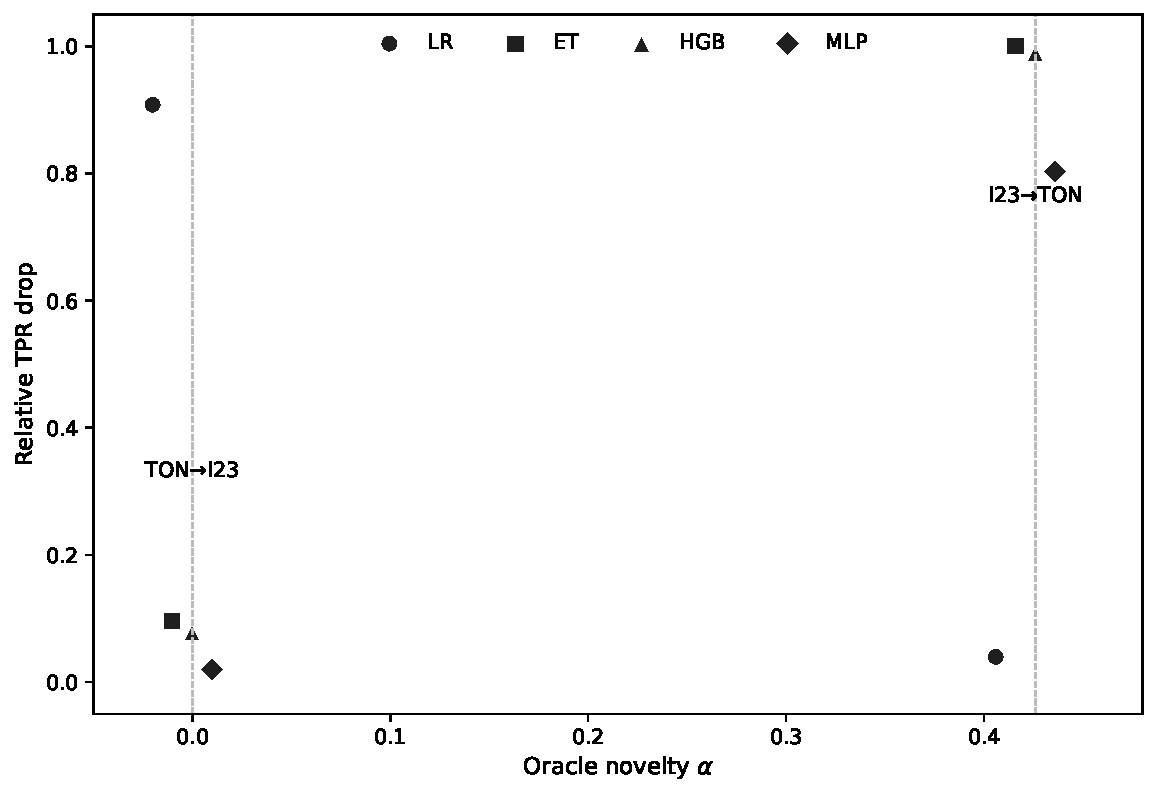
\includegraphics[width=0.9\textwidth]{figures/oracle_novelty_primary.pdf}
\caption{Oracle novelty versus relative TPR drop on the Tier~2 claim-bearing IoT subset. The figure is restricted to rows where both source and target ontology coverage meet the \NoveltyCoverageFloor{} rule.}
\label{fig:oracle-novelty}
\end{figure}

% Generated by scripts/41_build_manuscript_assets.py
\begin{table}[htbp]
\centering
\small
\setlength{\tabcolsep}{4pt}
\caption{Claim-bearing IoT subset used for the oracle novelty interpretation. The direction break is shown explicitly because the novelty reading is limited to these rows.}
\label{tab:primary-oracle-context}
\resizebox{\textwidth}{!}{%
\begin{tabular}{lllrrrrl}
\toprule
Source & Target & Model & Oracle $\alpha$ & Relative TPR drop & TPR@\FrozenFprTarget{} & Realized FPR & Catastrophic \\
\midrule
IoT-23 & ToN-IoT & LR & 0.426 & 0.040 & 0.500 & 0.189 & 1 \\
 &  & ET & 0.426 & 1.000 & 0.000 & 0.000 & 1 \\
 &  & HGB & 0.426 & 0.990 & 0.010 & 0.006 & 0 \\
 &  & MLP & 0.426 & 0.803 & 0.152 & 0.178 & 1 \\
\midrule
ToN-IoT & IoT-23 & LR & 0.000 & 0.908 & 0.007 & 0.040 & 0 \\
 &  & ET & 0.000 & 0.096 & 0.900 & 0.875 & 1 \\
 &  & HGB & 0.000 & 0.078 & 0.915 & 0.835 & 1 \\
 &  & MLP & 0.000 & 0.020 & 0.948 & 0.831 & 1 \\
\bottomrule
\end{tabular}
}
\end{table}


\FloatBarrier

\subsection{Benign Covariate Shift and False-Positive Drift}
\label{sec:covariate-shift}

The previous subsection analyzed attack novelty as a predictor of TPR drop. But the benchmark also shows substantial false-positive drift, which cannot be explained by attack-label novelty alone. This subsection analyzes benign covariate shift---distributional drift in the feature values of benign traffic---as a separate driver of false-positive inflation.

For each of the \DirectionCount{} ordered directions, we compute per-feature Kolmogorov--Smirnov (KS) test statistics between the source-holdout and target benign traffic distributions. The aggregate mean KS statistic summarizes how different the benign feature distributions are across domains.

The IoT-23~$\leftrightarrow$~ToN-IoT pair shows moderate benign covariate shift (mean KS~$\approx$~\IotPairMeanKs{}), while directions involving UNSW-NB15 show large benign covariate shift (mean KS~$\approx$~\UnswDirectionMeanKsMin{}--\UnswDirectionMeanKsMax{}). The IoT-23~$\to$~ToN-IoT and ToN-IoT~$\to$~IoT-23 directions have \emph{identical} benign covariate shift (the KS statistic is symmetric) but sharply different outcomes: the first direction has high attack novelty and dominant sensitivity loss, while the second has zero attack novelty but massive false-positive drift (mean realized FPR~$\approx$~\TonToIotMeanRealizedFpr{}). This two-direction contrast is consistent with attack novelty aligning more with sensitivity loss while benign shift interacts with the learned representation to produce false-positive drift.

At the direction level, however, the Spearman correlation between mean benign KS and FPR severity is $\DirectionBenignKsFprSeveritySpearman{}$ (weak, n=\DirectionCount{}), so the current data do not support a monotone global claim that larger benign shift yields larger false-positive inflation. The separability reading is therefore bounded to the directional contrast rather than a general law.

\FloatBarrier

\subsection{Deployable Monitor Comparison}

This subsection answers the deployable question directly. The target-free monitoring comparison does not support a main claim for $\hat{\alpha}$.

On all natural-transfer settings, $\hat{\alpha}$ reaches catastrophic-failure AUROC \AlphaHatAllNaturalCatastrophicAuroc{}, catastrophic-failure AUPRC \AlphaHatAllNaturalCatastrophicAuprc{}, and Spearman association with operational severity \AlphaHatAllNaturalSeveritySpearman{}. These effect sizes remain weak in absolute terms, and $\hat{\alpha}$ does not beat the strongest audited comparator on the full Tier~1 benchmark.

The same conclusion holds after the view is narrowed to the Tier~2 IoT subset. There, $\hat{\alpha}$ reaches catastrophic-failure AUROC \AlphaHatPrimaryCatastrophicAuroc{} and severity association \AlphaHatPrimarySeveritySpearman{}, which is better than its full-benchmark behavior but still too narrow a success to carry the monitoring story. The monitor comparison table therefore remains as a negative deployable result showing that no tested monitor, including composite aggregations of all four monitors, is ready for operational trust.

\begin{figure}[t]
\centering
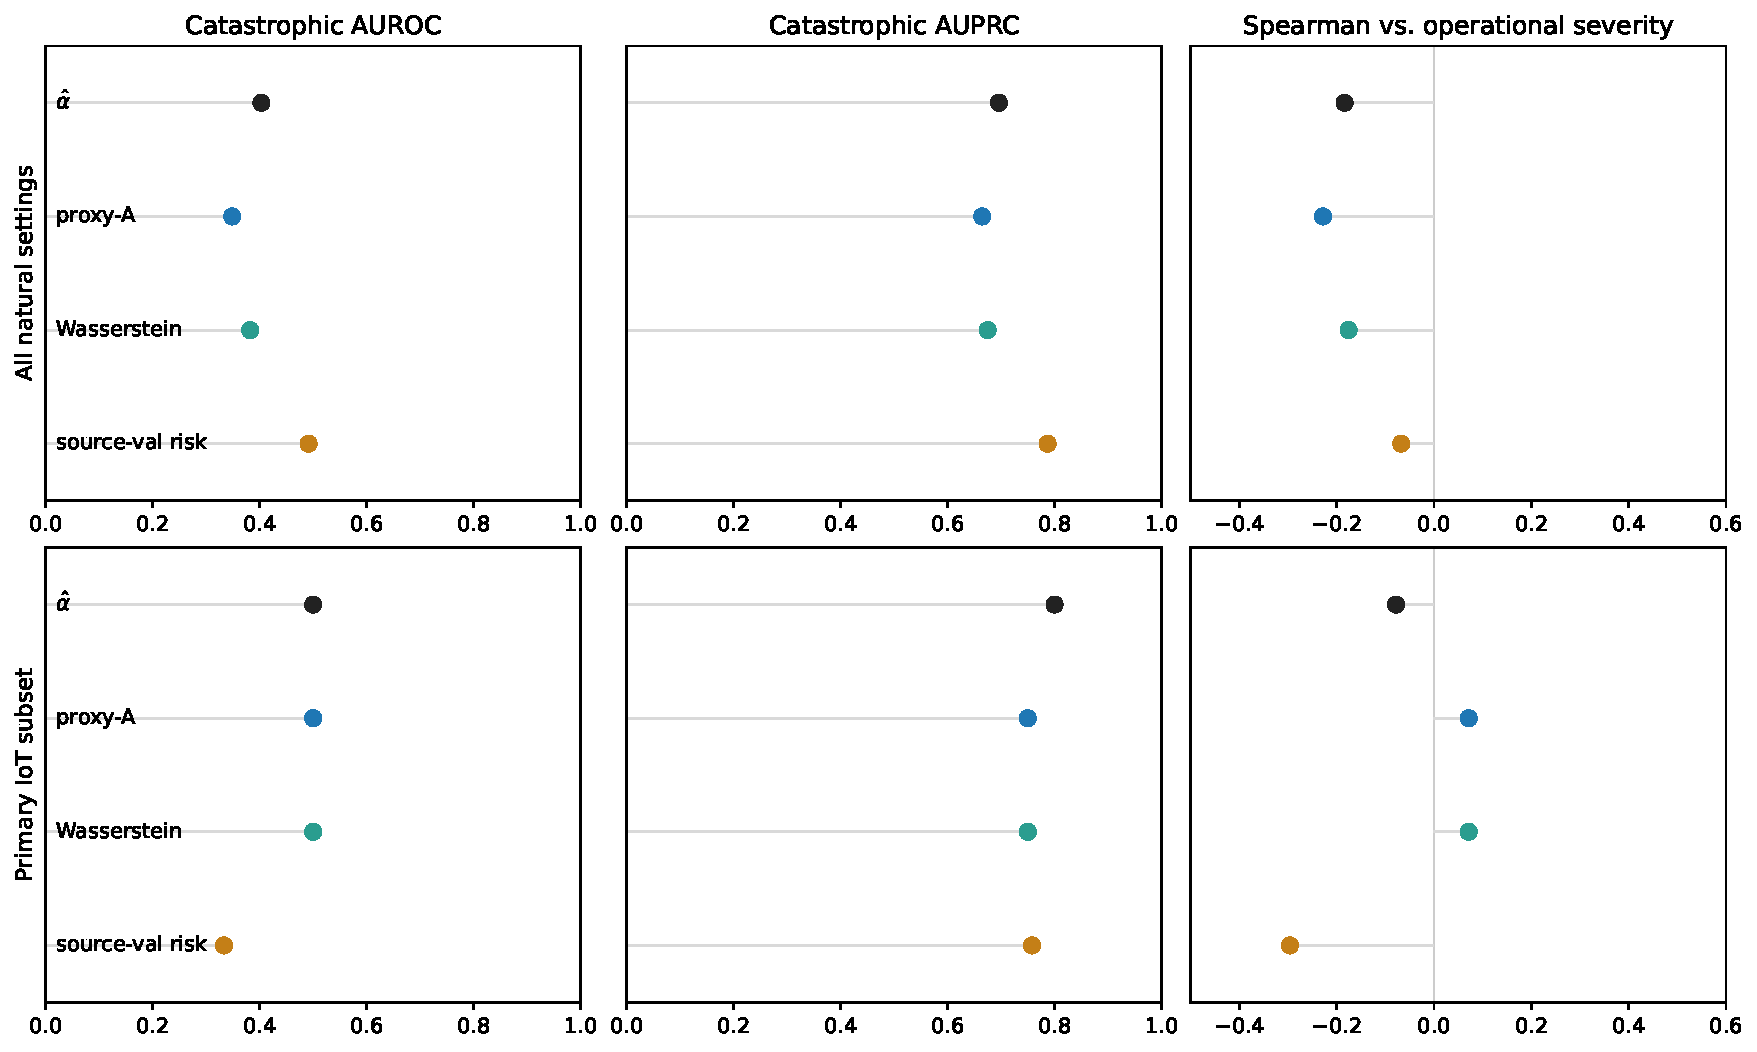
\includegraphics[width=\textwidth]{figures/monitor_comparison.pdf}
\caption{Deployable monitor comparison. The figure shows whether any tested monitor---including $\hat{\alpha}$, proxy-A distance, Wasserstein distance, and source-validation risk---becomes strong enough to support a deployable claim. None does.}
\label{fig:monitor-comparison}
\end{figure}

% Generated by scripts/41_build_manuscript_assets.py
\begin{table}[htbp]
\centering
\footnotesize
\setlength{\tabcolsep}{4pt}
\caption{Deployable monitor comparison derived directly from the canonical benchmark settings. Higher values indicate stronger alignment with operational severity and with catastrophic operational failure.}
\label{tab:monitor-comparison}
\resizebox{\textwidth}{!}{%
\begin{tabular}{llrrrlll}
\toprule
Subset & Score & Spearman vs. operational severity & Catastrophic AUROC & Catastrophic AUPRC & AUROC rank & AUPRC rank & Spearman rank \\
\midrule
all natural & $\hat{\alpha}$ & -0.184 & 0.403 & 0.696 & 2 & 2 & 3 \\
all natural & proxy-A & -0.228 & 0.349 & 0.665 & 4 & 4 & 4 \\
all natural & Wasserstein & -0.176 & 0.382 & 0.675 & 3 & 3 & 2 \\
all natural & source-val risk & -0.067 & 0.492 & 0.787 & 1 & 1 & 1 \\
\midrule
primary IoT & $\hat{\alpha}$ & -0.078 & 0.500 & 0.800 & 1 & 1 & 3 \\
primary IoT & proxy-A & 0.071 & 0.500 & 0.750 & 1 & 3 & 1 \\
primary IoT & Wasserstein & 0.071 & 0.500 & 0.750 & 1 & 3 & 1 \\
primary IoT & source-val risk & -0.296 & 0.333 & 0.758 & 4 & 2 & 4 \\
\bottomrule
\end{tabular}
}
\end{table}


\FloatBarrier

\section{Discussion}

The failure mode decomposition is the central analytical contribution of this paper. Prior cross-dataset IDS evaluations document that performance drops, but they do not distinguish ranking failure from threshold drift. That distinction has direct operational consequences: collapse, including the below-chance inversion case, cannot be repaired without retraining or domain adaptation, while threshold drift is in principle repairable with access to unlabeled target statistics. In this benchmark, \FullRankingFailureCount{} of \NaturalSettingCount{} settings fall into ranking failure, and on point estimates \FullInversionCount{} of those failing settings fall below chance. The dominant failure is therefore in the learned representation rather than in the operating-point calibration. This conclusion is not a single-threshold artifact: even at 5\%, competent-set median realized target FPR remains \BudgetFivePctCompetentMedianBudgetMultiple{}x the selected budget and \BudgetFivePctCompetentCatastrophicCount{} of \CompetentSettingCount{} settings remain catastrophic.

The covariate--novelty separation further refines the diagnostic picture, but only in a bounded way. The IoT-23~$\leftrightarrow$~ToN-IoT pair provides a useful two-direction contrast: both directions share the same benign covariate shift, but differ sharply in attack novelty. The higher-novelty direction (IoT-23~$\to$~ToN-IoT) degrades primarily in sensitivity, while the zero-novelty reverse direction degrades primarily in false-positive inflation. Across all \DirectionCount{} directions, however, the benign KS versus FPR-severity association is weak and negative (\DirectionBenignKsFprSeveritySpearman{}), so the current data do not support a monotone global law. The contrast is therefore suggestive rather than broadly predictive.

The monitor comparison narrows the deployable claims further. On the canonical full-data benchmark, $\hat{\alpha}$ remains non-deployable and does not outperform the strongest audited comparator on the full benchmark. Two design limitations matter here: by construction $\hat{\alpha}$ only sees attack-side novelty and is blind to benign shift, and its zero-positive fallback selects the top-$K$ target instances by detector score, coupling the estimate to the detector's own confidence calibration. That coupling is a known failure mode in OOD detection and may contribute to the proxy's weakness.

The results should not be read as evidence that cross-domain tabular flow-level NIDS transfer is universally infeasible. The benchmark uses a deliberately constrained shared feature schema that trades model capacity for comparability. Richer feature representations, payload-aware architectures, or domain-adaptation methods may fare differently under the same protocol. The contribution is the decomposition methodology and the specific empirical characterization, not a universal impossibility claim.

\section{Limitations}

The novelty result is intentionally narrow. Only \PrimaryIotSettingCount{} settings satisfy the current ontology coverage rule, which requires mapped attack coverage of at least \NoveltyCoverageFloor{} on both source and target domains. The oracle novelty story therefore applies only to the Tier~2 IoT subset, not to the full three-dataset matrix.

UNSW-NB15 remains a stress-test domain rather than a semantic peer in the novelty analysis. Its directions belong in Tier~1 because they reveal transferred instability, but the current ontology does not justify using those rows as evidence for the novelty claim. The study also uses one aggressively reduced shared tabular feature schema. That keeps the benchmark comparable, but it likely discards useful signal that richer dataset-native feature sets retain. To make that limitation explicit, the repository now includes an auxiliary within-domain information-retention audit comparing the canonical shared-16 representation against dataset-native augmented feature sets; those results are diagnostic only and are not mixed into the cross-dataset transfer benchmark because the native spaces are not directly comparable across datasets. The auxiliary audit is also HGB-only, so it should be read as a representative strong-model diagnostic rather than evidence that LR / ET / MLP retain the same amount of dataset-native signal. The study also does not include sequence-based NIDS baselines. Their transfer behavior under the same protocol remains outside scope.

% Generated by src/iot_ids/native_auxiliary.py
\begin{table}[!htbp]
\centering
\footnotesize
\setlength{\tabcolsep}{2pt}
\caption{Auxiliary within-domain information-retention audit. The canonical shared-16 representation is compared with a dataset-native augmented representation that adds admissible local fields and summarized endpoint features. HGB is shown as one representative strong shared-schema model; this HGB-only audit does not establish the same retention behavior for LR / ET / MLP. These native features are dataset-specific and are not used in the cross-dataset transfer benchmark.}
\label{tab:native-feature-aux}
\resizebox{\textwidth}{!}{%
\begin{tabular}{@{}llcccccc@{}}
\toprule
Dataset & Model & \begin{tabular}[c]{@{}c@{}}Shared\\feat.\end{tabular} & \begin{tabular}[c]{@{}c@{}}Native\\feat.\end{tabular} & \begin{tabular}[c]{@{}c@{}}Shared\\AUROC\end{tabular} & \begin{tabular}[c]{@{}c@{}}Native\\AUROC\end{tabular} & \begin{tabular}[c]{@{}c@{}}$\Delta$\\AUROC\end{tabular} & \begin{tabular}[c]{@{}c@{}}$\Delta$\\TPR@1\%\end{tabular} \\
\midrule
IoT-23 & HGB & 16 & 24 & 0.988 & 0.988 & 0.000 & -0.001 \\
ToN-IoT & HGB & 16 & 38 & 1.000 & 1.000 & 0.000 & 0.005 \\
UNSW-NB15 & HGB & 16 & 21 & 0.981 & 0.981 & 0.000 & 0.000 \\
\bottomrule
\end{tabular}
}
\end{table}


The ontology coverage threshold of \NoveltyCoverageFloor{} determines which settings enter Tier~2. This value was fixed before the benchmark was read. A sensitivity sweep shows that the Tier~2 subset is identical for all coverage floors from \CoverageSweepStableFloorMin{} to \CoverageSweepStableFloorMax{} (the same \PrimaryIotSettingCount{} IoT-only settings pass at every threshold in this range), collapsing to an empty set only at \CoverageSweepEmptyFloor{}. The threshold choice therefore does not affect the novelty analysis within the reasonable range.

The target-free monitoring comparison is bounded as well. The $\hat{\alpha}$ proxy's zero-positive fallback introduces a dependency on the detector's confidence calibration under shift, which is a known failure mode. Even with this acknowledged, no alternative fallback strategy tested (random sampling of target instances) materially changes the result. Operational severity is a stylized summary rather than a full cost model for analyst workload. Even under this operational target, no monitor in this study establishes a generally deployable safety signal.

\section{Conclusion}

This paper contributes a failure mode decomposition for fixed-threshold tabular flow-level NIDS transfer, distinguishing ranking failure from threshold drift and separating attack-novelty effects from benign covariate shift. Across \DirectionCount{} ordered directions, \ModelCount{} tabular models, and \NaturalSettingCount{} transfer settings in this three-corpus benchmark, the dominant failure is ranking failure (\FullRankingFailureCount{} of \NaturalSettingCount{} settings). On point estimates, \FullInversionCount{} of those failing settings fall below chance and therefore indicate inverted target score orientation under the transferred rule. This central result is robust to the 0.5\%/1\%/5\% source-side budget sweep: even at 5\%, competent-set median realized target FPR remains \BudgetFivePctCompetentMedianBudgetMultiple{}x the selected budget and \BudgetFivePctCompetentCatastrophicCount{} of \CompetentSettingCount{} settings remain catastrophic, still \BudgetFivePctCompetentCatastrophicShare{} of the competent set. A split-matched auxiliary CORAL check raises whole-ROC AUROC but leaves low-FPR ranking unchanged and worsens off-budget/catastrophic behavior. Oracle novelty provides only a bounded directional interpretation on the \PrimaryIotSettingCount{} claim-bearing IoT rows, while the benign-shift story remains a two-direction contrast plus a weak global KS relation rather than a general predictor. The pre-registered target-free novelty proxy remains a negative result rather than a deployable monitor. Taken together, these results support a stricter diagnostic framework for evaluating benchmark-bounded cross-dataset tabular flow-level NIDS deployment and identify the ranking-versus-threshold decomposition as a necessary first step before attempting transfer repair.

\appendix
\section{Diagnostic Oracle Retuning}
\label{app:oracle-retuning}

This appendix reports the diagnostic target-retuned threshold summary generated directly from the canonical artifacts. The retuned thresholds use target labels at the same \FrozenFprTarget{} budget for diagnosis only; they are not part of the frozen-threshold benchmark protocol.

% Generated by scripts/41_build_manuscript_assets.py
\begin{table}[htbp]
\centering
\scriptsize
\setlength{\tabcolsep}{4pt}
\caption{Diagnostic oracle retuning at the same \FrozenFprTarget{} false-positive budget. Thresholds are re-selected with target labels for diagnosis only; this table is not part of the frozen-threshold benchmark protocol. The change column reports the median of per-setting retuned-minus-fixed TPR changes within each direction, not the difference between direction medians. When the transferred frozen threshold already runs far above the target-domain \FrozenFprTarget{} FPR budget, oracle retuning must raise the cutoff to restore that budget; if target ranking is weak, that corrected cutoff can collapse TPR.}
\label{tab:oracle-retuned-summary}
\begin{tabular}{lrrr}
\toprule
Direction & Fixed TPR & Retuned TPR & Median paired $\Delta$TPR \\
\midrule
I23$\to$TON & 0.081 & 0.037 & -0.048 \\
I23$\to$UNSW & 0.197 & 0.006 & -0.192 \\
TON$\to$I23 & 0.907 & 0.001 & -0.907 \\
TON$\to$UNSW & 0.233 & 0.000 & -0.232 \\
UNSW$\to$I23 & 0.042 & 0.020 & 0.000 \\
UNSW$\to$TON & 0.022 & 0.001 & -0.021 \\
\bottomrule
\end{tabular}
\end{table}

\FloatBarrier

\section*{Funding}

Funding information will be added at submission.

\section*{Declaration of competing interest}

The authors declare that they have no known competing financial interests or personal relationships that could have appeared to influence the work reported in this paper.

\section*{Data availability}

Dataset sources and generated benchmark artifacts are described in the repository. A formal data-availability statement will be added at submission.

\bibliographystyle{elsarticle-num}
\bibliography{references}

\end{document}
